\documentclass{article}
\usepackage[danish]{babel}
\usepackage{graphicx}
\usepackage{listings}
\usepackage[utf8]{inputenc}
\usepackage{biblatex}
\usepackage{xcolor}
\usepackage{multirow}
\newcommand\myworries[1]{\textcolor{red}{#1}}
\addbibresource{sample.bib}
\title{My final report}
\usepackage[utf8]{inputenc}
\author{Emil Skovbo}
\date{ }
\begin{document}
\clearpage
\maketitle
\thispagestyle{empty}

\tableofcontents
\section{Introduction}

Lorem ipsum dolor sit amet, consectetur adipiscing elit. Cras risus ligula, bibendum cursus vulputate in, varius eu enim. Praesent scelerisque nulla nec facilisis elementum. Cras aliquet, orci eu ornare pulvinar, odio metus aliquam erat, ut facilisis odio sapien vitae sapien. Phasellus quis ante eget orci commodo mattis. Quisque dictum, elit vitae tincidunt tincidunt, metus massa condimentum libero, eget sagittis nulla nunc sit amet ex. Vivamus mi dolor, lobortis et tempor vel, scelerisque nec eros. Maecenas ut viverra lorem. Ut mi tortor, consectetur quis efficitur vitae, gravida nec eros. Integer tempor elit vel nunc fermentum, a facilisis orci vestibulum. Integer vel erat at libero semper scelerisque.



Ut rhoncus egestas faucibus. Ut ultricies, augue sed hendrerit varius, arcu nisl tincidunt turpis, quis faucibus purus nisl sit amet justo. Curabitur nisi massa, tincidunt sit amet mollis id, consectetur sed tellus. Vestibulum aliquet, nulla at commodo scelerisque, orci massa finibus felis, id feugiat massa justo at libero. Mauris commodo purus ut erat porttitor, nec condimentum tortor auctor. Aenean vitae diam quis diam sollicitudin ultrices. In malesuada urna ac ornare egestas. Integer ullamcorper blandit metus, ac vehicula arcu pulvinar in. Sed in scelerisque quam. Aenean pharetra ullamcorper orci ac luctus. Sed ante eros, pretium quis nunc ullamcorper, venenatis laoreet eros.

Aenean ultricies arcu sem, ac interdum ipsum rhoncus quis. Nullam eget nisl sed massa ultrices pretium. Proin pulvinar massa odio, ac hendrerit sapien maximus sit amet. Phasellus odio ante, pellentesque ut lorem et, varius facilisis quam. Cras imperdiet auctor nulla, faucibus vestibulum nulla rhoncus non. Morbi gravida enim quis convallis molestie. Phasellus maximus venenatis neque, at ornare purus. Curabitur consequat, purus at volutpat pretium, leo neque consequat lectus, id semper eros urna et sapien. Nulla convallis purus leo, non consequat nibh ullamcorper in. Etiam interdum felis eu erat posuere bibendum. Praesent eget nulla quis sapien vulputate hendrerit cursus ut sapien. Suspendisse cursus non libero eget lacinia. Sed sit amet rutrum ex. Phasellus eget faucibus leo, non cursus neque. Cras facilisis turpis turpis, quis consequat quam bibendum eu.

Cras accumsan, leo et rhoncus mattis, quam arcu lobortis arcu, id luctus purus ante non felis. Curabitur dapibus, nulla sed pulvinar dictum, nisl odio venenatis odio, aliquam faucibus dui leo id felis. Nulla posuere porttitor sem, ac varius nisi scelerisque eget. Integer tristique tortor vitae vehicula ullamcorper. Vivamus maximus lacus justo, nec ornare risus pellentesque at. Vivamus in purus iaculis, egestas elit at, consectetur erat. Fusce in dolor mauris. Sed nec sem finibus, efficitur dui at, lacinia mi. Mauris auctor arcu ut arcu molestie porta.
\subsection{Sub-intro}
Fusce molestie velit id massa tempus, nec congue urna sagittis. Vivamus feugiat mollis felis, lacinia volutpat libero pretium nec. Integer porta imperdiet ligula ut consectetur. Aliquam sapien leo, porttitor eu turpis vel, faucibus cursus arcu. Donec scelerisque bibendum magna et venenatis. Vestibulum in convallis urna. Nulla malesuada rutrum diam, ut volutpat nisi ullamcorper ut. Aenean cursus purus id pharetra viverra. In ornare, nulla ac posuere rutrum, nibh magna convallis mauris, eu lacinia dolor nisl sit amet magna. Donec sit amet molestie neque. Sed luctus placerat dolor, ac sagittis arcu lobortis vel. Vivamus a libero feugiat, pretium turpis in, condimentum elit. Donec est risus, hendrerit sit amet malesuada sed, semper pulvinar nisi. Vestibulum pretium, quam ut scelerisque elementum, nibh sem ullamcorper elit, vitae aliquam eros lorem vitae nunc. Cras sit amet tortor pharetra eros auctor pretium eget non ante.
\subsubsection{Sun-Sub section}

Let's cite! The Einstein's journal paper \cite{einstein} and the Dirac's 
book \cite{dirac} are physics related items. 

\printbibliography




This is the text in first paragraph. This is the text in first 
paragraph. This is the text in first paragraph. \par
This is the text in second paragraph. This is the text in second 
paragraph. This is the text in second paragraph.

\section*{Non-numbered section} 
 
\begin{figure}[htp]
    \caption{A picture of a page.}
    \centering
    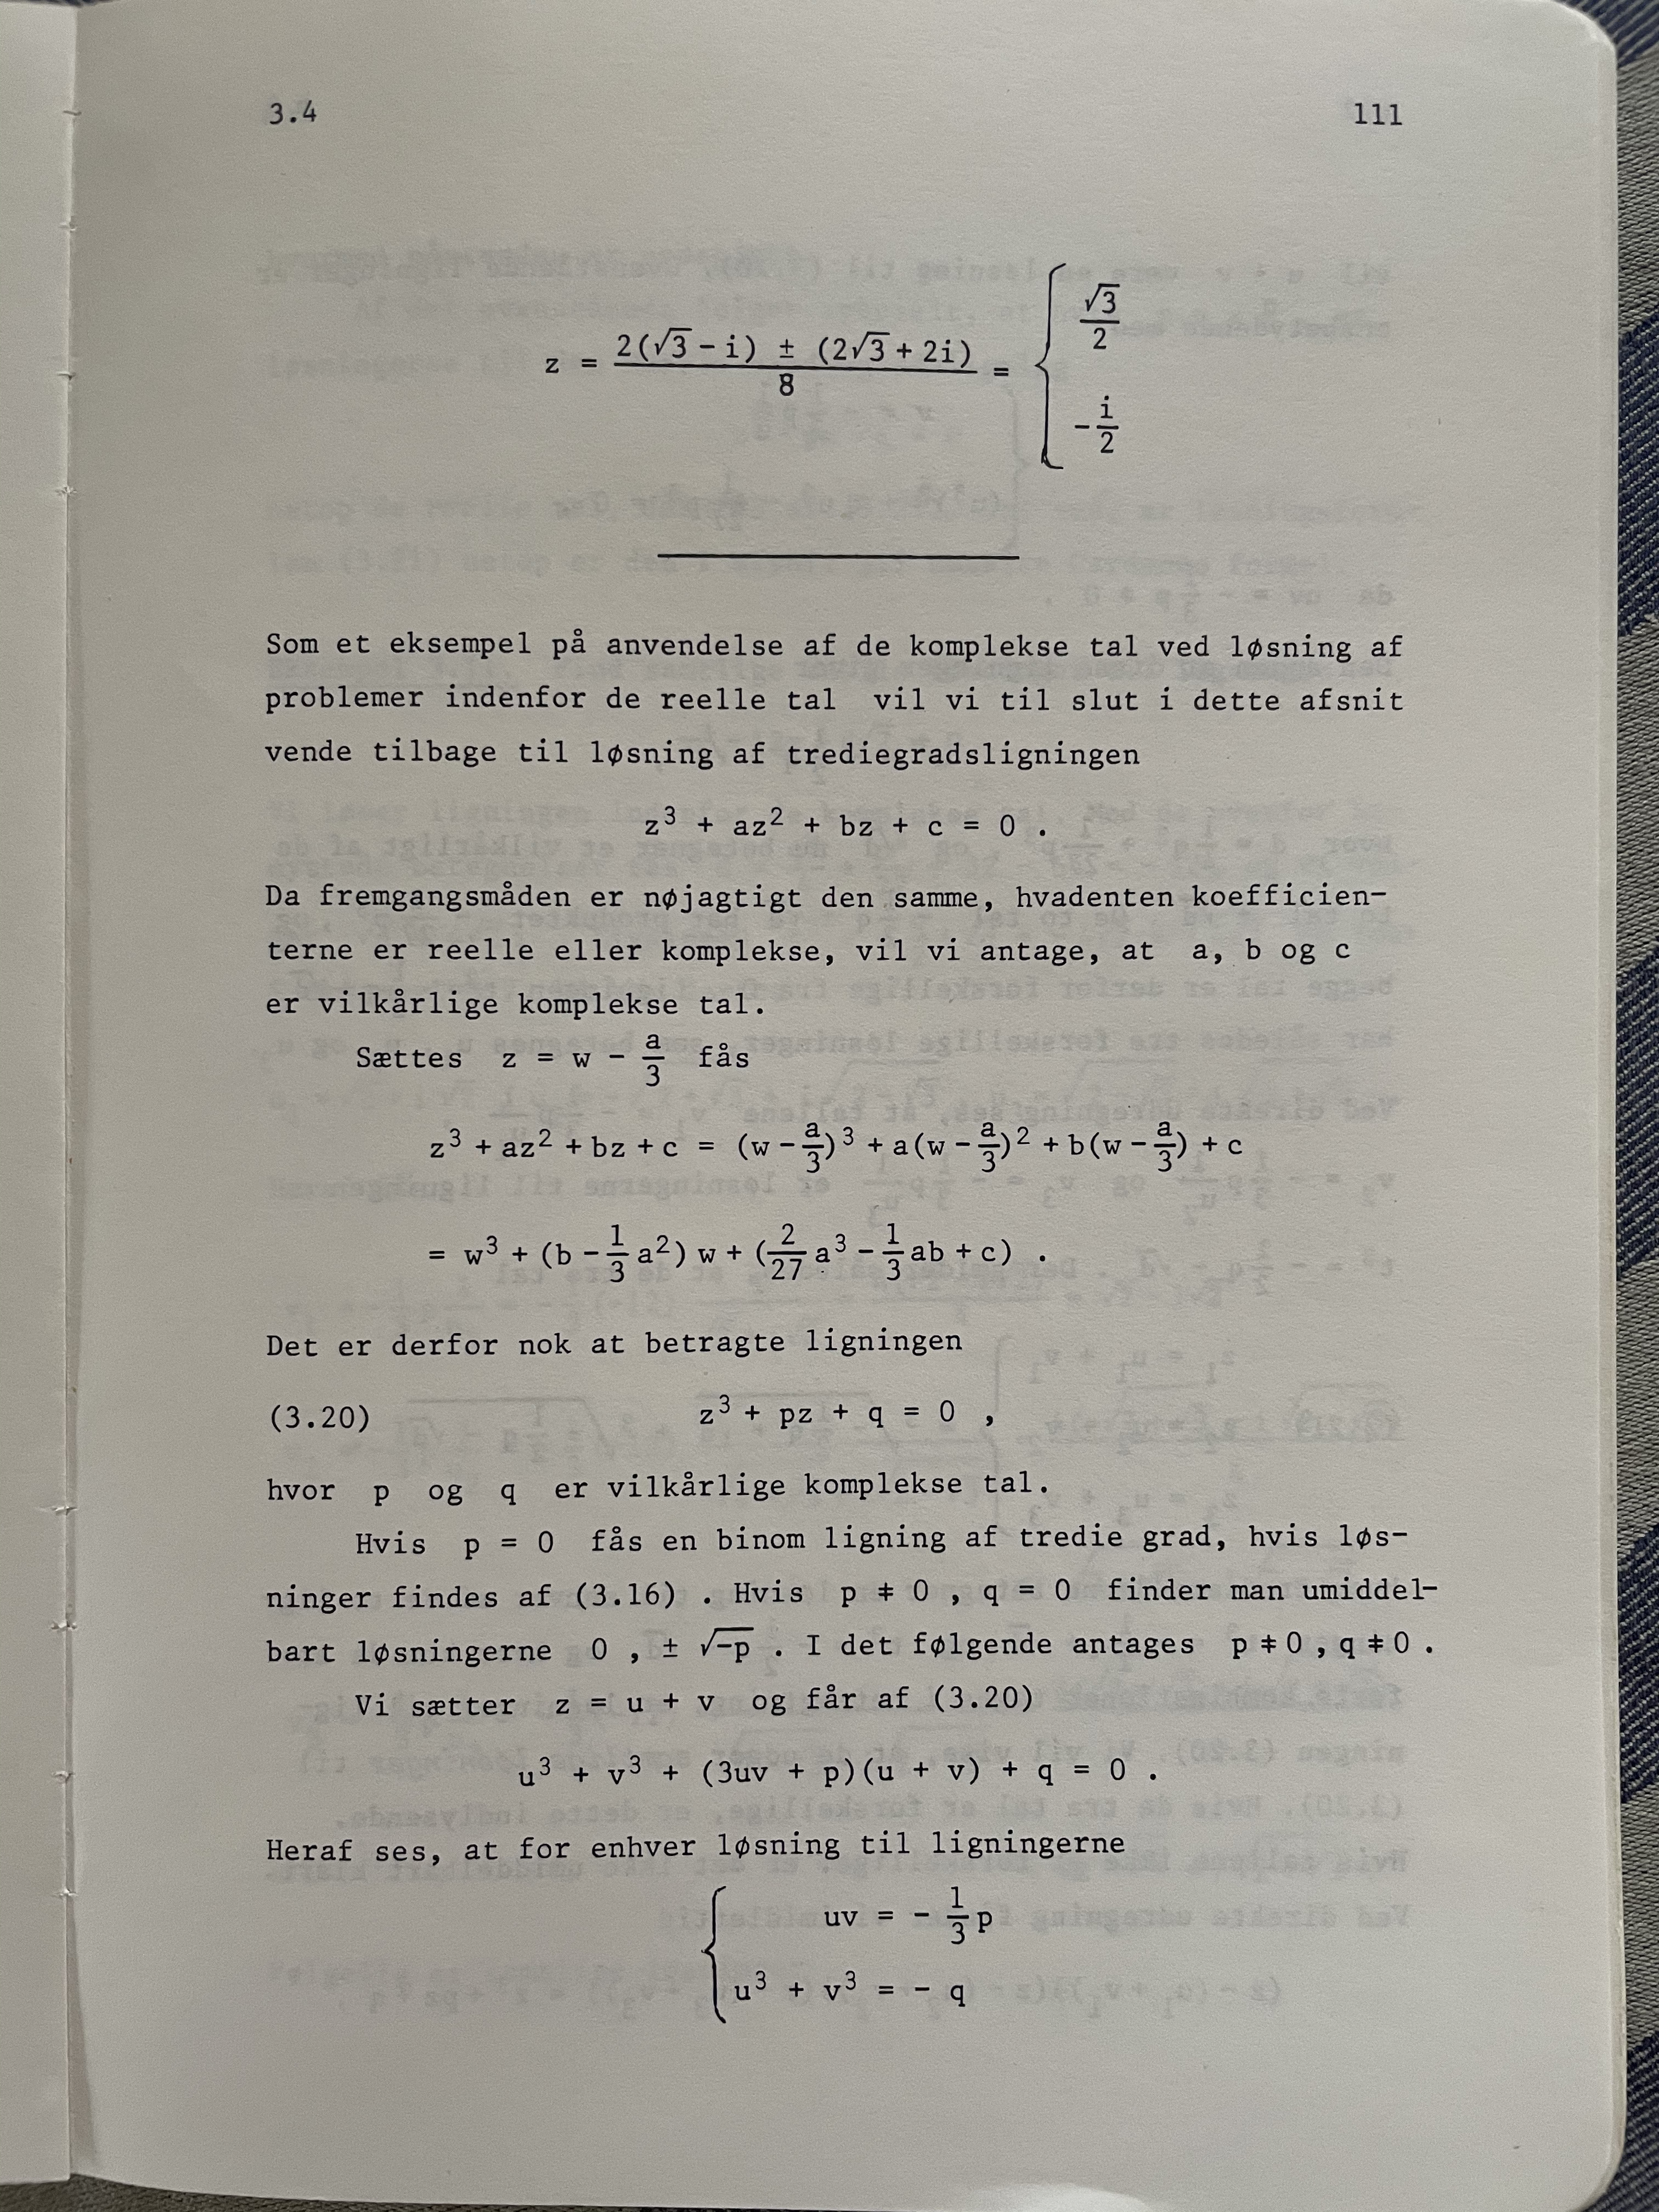
\includegraphics[width=4cm]{image.png}
    \includegraphics[width=4cm]{stego.png}
    \caption{An image of cph}
    \label{fig:galaxy}
\end{figure}

\begin{itemize}
  \item The individual entries are indicated with a black dot, a so-called bullet.
       \begin{itemize}
        \item  Second Level
    \end{itemize}
  \item The text in the entries may be of any length.
\end{itemize}

\renewcommand{\labelenumii}{\Roman{enumii}}
\begin{enumerate}
   \item First level item
   \item First level item
   \begin{enumerate}
     \setcounter{enumii}{4}
     \item Second level item
     \item Second level item
       \begin{enumerate}
       \item Third level item
       \item Third level item
         \begin{enumerate}
         \item Fourth level item
         \item Fourth level item
       \end{enumerate}
     \end{enumerate}
   \end{enumerate}
 \end{enumerate}


\section{Introduction}
   
This is the first section.
Lorem  ipsum  dolor  sit  amet,  consectetuer  adipiscing  
elit.   Etiam  lobortisfacilisis sem.  Nullam nec mi et 
neque pharetra sollicitudin.  Praesent imperdietmi nec ante. 
Donec ullamcorper, felis non sodales...
       
\addcontentsline{toc}{section}{Unnumbered Section}
\section*{Unnumbered Section}

Lorem ipsum dolor sit amet, consectetuer adipiscing elit.  
Etiam lobortis facilisissem.  Nullam nec mi et neque pharetra 
sollicitudin.  Praesent imperdiet mi necante...

\section{Second Section}
       
Lorem ipsum dolor sit amet, consectetuer adipiscing elit.  
Etiam lobortis facilisissem.  Nullam nec mi et neque pharetra 
sollicitudin.  Praesent imperdiet mi necante...
  
\ref{fig:galaxy}

Please see Figure ~\ref{fig:galaxy} for a prototype yada yada yada
       
       
       
       
\begin{lstlisting}
import numpy as np
    
def incmatrix(genl1,genl2):
    m = len(genl1)
    n = len(genl2)
    M = None #to become the incidence matrix
    VT = np.zeros((n*m,1), int)  #dummy variable
    
    #compute the bitwise xor matrix
    M1 = bitxormatrix(genl1)
    M2 = np.triu(bitxormatrix(genl2),1) 

    for i in range(m-1):
        for j in range(i+1, m):
            [r,c] = np.where(M2 == M1[i,j])
            for k in range(len(r)):
                VT[(i)*n + r[k]] = 1;
                VT[(i)*n + c[k]] = 1;
                VT[(j)*n + r[k]] = 1;
                VT[(j)*n + c[k]] = 1;
                
                if M is None:
                    M = np.copy(VT)
                else:
                    M = np.concatenate((M, VT), 1)
                
                VT = np.zeros((n*m,1), int)
    
    return M
\end{lstlisting}
       
       
       
       
\[ x^n + y^n = z^n \]

The mass-energy equivalence is described by the famous equation

\[E=mc^2\]

discovered in 1905 by Albert Einstein. 
In natural units ($c$ = 1), the formula expresses the identity

\begin{equation}
E=m
\end{equation}



\begin{table}[ht]
\caption{Multi-column and multi-row table}
\begin{center}
\begin{tabular}{ccc}
    \hline
    \multicolumn{2}{c}{\multirow{2}{*}{Multi-col-row}}&X\\
    \multicolumn{2}{c}{}&X\\
    \hline
    X&X&X\\
    \hline
\end{tabular}
\end{center}
\label{tab:multicol}
\end{table}

\begin{table}[ht]
\caption{Partial horizontal line}
\begin{center}
\begin{tabular}{ccc}
    \hline
    \multicolumn{2}{c}{Multi-column}&\\
    \cline{1-2}
    X&X&X\\
    X&X&X\\
    \hline
\end{tabular}
\end{center}
\label{tab:multicol}
\end{table}


\myworries{to do notes}
       
\end{document}